%!TEX root = base.tex

\chapter{Experimental Methodology}

This chapter describes rationale for the experimental approach used to evaluate
the theoretical models.

To evaluate the theoretical model there must first exist some set of values
produced by the model itself, and an equivalent set of data to compare against.
In this report, the values produced by the model are referenced to as
\emph{model parameters}. The other set of data, the comparison set, is gathered
from a specific device, the TG799-VAC, and referred to as the \emph{router
metrics}.

The general methodology of the model evaluation consists of iteration between
selection of model parameters and router metrics until both datasets could be
compared. Metrics were in most cases also analysed if they behaved as expected,
were accurate or precise.

\section{Model Parameters}
The first step was to analyse the theoretical models.

A python implementation of the Felemban-Ekici model can be found in listing
\ref{lst:efmodel} and requires a set of constants, specified below:

\begin{itemize}
	\item \emph{N}, the number of network nodes
	\item $CW_{min}$ and $CW_{max}$, contention window min and max size
	\item \emph{E[D]}, the mean payload size
	\item channel bit rate
	\item $L$, the \texttt{ShortRetryLimit}
\end{itemize}

The Felemban-Ekici model provides normalized throughput ($U$), channel access
delay and probability of packet collision. However, after implementing the
model, severe differences regarding the normalized throughput were discovered.
While the re-implementation achieves packet collision probabilities similar to
the original paper, no realistic tuning of throughput calculation parameters
could reproduce the original values found in the paper. Thus this value is not
generated by the re-implemented model, but rather compared to the curves found
in the paper.

\section{Experimental Model Evaluation}

A study of the networking stack revealed an approach of how to measure backoff times.

\section{Parameter Mapping}  

As mentioned, experiments were performed using \texttt{jana} to set packet
rates and payload sizes, and \texttt{ubus} to interact with the router
firmware to retrieve data.

\section{Model Evaluation with Real-World Data}

The second round of model evaluation was based on data from end users. This
required tools for accessing the network interface statistics, matching a set of
\emph{router metrics} with the \emph{model parameters} and analysis of the
selected \emph{router metrics} to guard against bugs.

\subsection{Interface}

Network interface data can be accessed through various different interfaces. In
this thesis two programs were tried during exploratory testing, \texttt{ubus}
and \texttt{quantenna api}. In the end \texttt{ubus} was chosen due to its
broader range of statistics (both 2.4 and 5.0 GHz modems) and consistency of its
output (no corrupt/invalid JSON was found).

\subsection{Metrics}
Selecting a set of metrics which are equivalent to the model parameters.

This required a good understanding oh how the constraints of the model affected
the selection of router metrics, e.g. the model separates CTS-RTS and Basic mode
while the router automatically decides which to use based on packet payload
size, which isn't available to any tool.

In order to evaluate the models we needed these metrics:

\begin{itemize}
\item rssi
\item nodes
\item logical tx/rx rates
\item physical tx/rx rates
\end{itemize}

\subsection{Metric analysis}

We must analyse the validity of the reported parameters.

Do this with experimentation in the radio lab.

We want to analyse the reported values for RSSI, SNR, broken \& valid IEEE
802.11 frames.

Using quantenna and wl API:s to query:
\begin{itemize}
    \item \texttt{ubus call wireless.radio.monitor get}
    \item \texttt{ubus call wireless.ssid.stats get}
    \item \texttt{ubus call wireless.radio.stats get}
\end{itemize}

\subsection{Traffic counters}

As noted above, one of the \emph{model parameters} is normalised throughput,
defined in \cite{felemban} as

\begin{equation}
U = \frac{P_{success}T_{payload}}{P_{success}T_{payload} + (P_{busy} -
P_{success})T_{collision} + (1 - P_{busy})T_{idle}}
\end{equation}

where $P_x$ is probability of $x$ and $T_y$ time of $y$, e.g. probability of successful transmission or time to send payload over channel.

There are no direct equivalent \emph{router metrics} available. Instead traffic counters such as $TX_{packets}$,
$RX_{packets}$, $TX_{bytes}$ and $RX_{bytes}$, are required to compute an average throughput, $N$

\begin{equation}
N = \frac{TX_{bytes} + RX_{bytes}}{t}
\end{equation}

\subsection{RSSI experiments}

Received Signal Strength Indicator (RSSI) is an important, and tricky, value. It
is important because it is often the only indicator of signal strength, and
tricky due to high variance between two chips, from same or different vendors,
suggesting that variance stems from a combination of hardware and software
factors \cite{lui}.

In order to establish whether the RSSI metric could be used or not, analysis had
to be done to verify the behavior, accuracy and variance of the reported values.
This was done in a shielded lab with low-to-no external interference and no self
interference from reflection.

Figure \ref{fig:rssi_setup} shows how the router, antenna and laptop were
set-up. Three experiment sessions were carried out to measure RSSI, about 5
minutes per session, with two different spectrum analysers.

The first test established the baseline rssi values when the system (laptop) was
idle, i.e. any network load originated from background services. The second test
was conducted using \texttt{iperf3} to push as much network load as possible,
see listings \ref{lst:router}, \ref{lst:client} and \ref{lst:rssi} for relevant
scripts. The third test was a control test with a different spectrum analyser,
but otherwise identical to the second test.

Scripts for parsing the spectrum analyser data and related heat map generator
are detailed in listings \ref{lst:mdrparse} and \ref{lst:mdrplot}.

The \emph{spectrum analyser data} was plotted as a heat map; frequency vs. time
vs. signal strength. This graph shows both how signal strength varies over time
and frequency. In contrast, the \emph{router metrics} only specify one RSSI
value and thus the resulting plot compares RSSI vs. time. The graphs can be
analysed individually for insight into system behavior and compared to see how
they relate.

\begin{figure}
\center
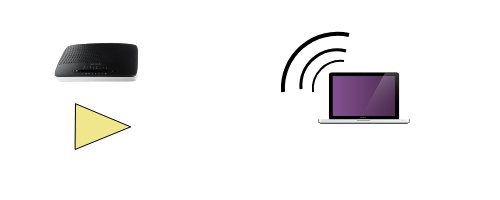
\includegraphics[width=0.9\textwidth]{images/rssi_setup.png}
\caption{TG799 router and measurement antenna side by side, 1 meter from laptop}
\label{fig:rssi_setup}
\end{figure}

\subsection{Evaluation}

Armed with a solid set of \emph{router metrics} data collection could begin.
Different scenarios were planned and tested.